\section{Method}
\label{sec:method}

\Cref{fig:arch} summarises \method{}. A frozen encoder produces camera-aware tokens for both views; a transformer decoder with joint and object queries drives two complementary estimators of the field, a direct regression head and a geometric head that predicts hand joints and the object pose and evaluates \cref{eq:field} through a differentiable nearest-vertex operator; the two are fused by their predicted precisions.

\begin{figure*}[t]
\centering
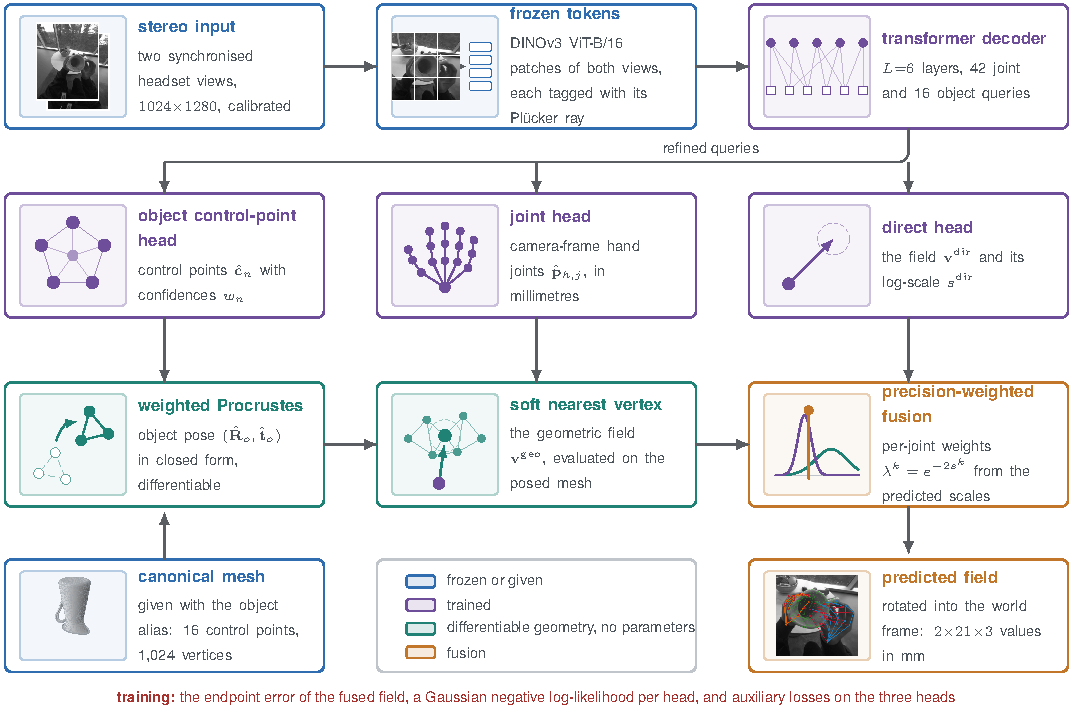
\includegraphics[width=\textwidth]{fig/architecture.pdf}
\caption{Overview of the factored interaction-field model, drawn on a held-out frame. First row: both views are encoded once by a frozen backbone and cached, every patch token is tagged with the Pl\"ucker coordinates of its pixel ray, and a decoder refines 42 joint queries and 16 object queries against the tokens of both views. Second row: three linear heads read those queries; the direct head regresses the field itself, while the joint head and the object control-point head supply the two arguments of $G$. Third row, each item under the head that feeds it: weighted Procrustes alignment turns the predicted control points into an object pose in closed form, the soft nearest-vertex operator evaluates the field on the mesh posed by it, so that every predicted endpoint lies on the object surface by construction, and the two field estimates are averaged with weights given by their own predicted precisions. Fourth row: the canonical mesh, which is given with the object alias, the colour key, and the output after rotation into the world frame. The auxiliary losses train the heads on frames that the field loss cannot use.}
\label{fig:arch}
\end{figure*}

\subsection{Camera-aware frozen tokens}
\label{sec:tokens}
Each view is resized to $480\times384$ and encoded by a frozen DINOv3 ViT-B/16~\cite{simeoni2025dinov3,oquab2024dinov2,dosovitskiy2021vit}, yielding $N{=}720$ patch tokens $\mathbf{X}_v\in\mathbb{R}^{N\times D}$ per view. Following GOLF~\cite{zou2026golf}, every token is tagged with the Pl\"ucker coordinates $\boldsymbol{\pi}(u,v)=[\mathbf{d},\,\mathbf{o}\times\mathbf{d}]\in\mathbb{R}^6$ of its pixel ray expressed in the reference camera, with unit direction $\mathbf{d}=\mathrm{normalize}(\Rot_{c\leftarrow v}\mathbf{K}_v^{-1}[u;1])$ and origin $\mathbf{o}$ in metres~\cite{sitzmann2021lfn}, so that stereo geometry enters the network explicitly:
\begin{equation}
  \mathbf{X}'_v = \mathbf{P}\mathbf{X}_v + \mathrm{MLP}(\boldsymbol{\pi}) + \mathbf{e}_{\text{view}}(v) + \mathbf{e}_{\text{pos}}.
  \label{eq:tokens}
\end{equation}
Here $\mathbf{P}$ projects the cached tokens to the decoder width, $\mathbf{e}_{\text{view}}$ is a learned view embedding and $\mathbf{e}_{\text{pos}}$ a learned positional embedding over the $30\times24$ token grid. The memory is the concatenation of both views' tokens (1440 tokens; 720 for single-view variants). Because the encoder is frozen, tokens are computed once and cached, which is what makes the study feasible on modest hardware; the design is agnostic to the encoder.

\subsection{Decoder and heads}
\label{sec:decoder}
Learned queries comprise $2J{=}42$ joint queries $\mathbf{z}_{h,j}$ and $N_o{=}16$ object queries $\mathbf{z}^o_n$, one per canonical control point $\mathbf{c}_n\in\mesh_a$ selected by farthest-point sampling~\cite{qi2017pointnetpp}; the object alias enters through an embedding added to the object queries. An $L$-layer decoder~\cite{vaswani2017attention} with self-attention over all queries and cross-attention to the memory refines them; the joint-query formulation follows DETR-style set prediction~\cite{carion2020detr} as adapted for hands by the winning ARCTIC entry~\cite{abouzeid2023jointtransformer}. Linear heads then predict the direct field and its log-scale, the camera-frame joints, and the object control points with confidences,
\begin{align}
  \field^{\text{dir}}_{h,j}&=\mathbf{W}_v\mathbf{z}_{h,j},\qquad s^{\text{dir}}_{h,j}=\mathbf{w}_s^{\top}\mathbf{z}_{h,j},\qquad \hat{\joint}_{h,j}=\mathbf{W}_p\mathbf{z}_{h,j},\\
  \hat{\mathbf{c}}_n&=\mathbf{W}_c\mathbf{z}^o_n,\qquad w_n=\mathrm{softmax}_n(\mathbf{w}_w^{\top}\mathbf{z}^o_n),
\end{align}
together with per-hand presence and per-joint visibility logits used only as auxiliary targets. Regression outputs are scaled by 100\,mm and joint predictions are offset by 300\,mm in depth so that the heads start near the data scale. Log-scales are clamped to $[-3,5]$, corresponding to standard deviations between 0.05 and 148\,mm; the upper bound turns out to matter in \cref{sec:inside}.

\subsection{Geometric field}
\label{sec:geo}
The object pose is obtained in closed form from the predicted control points by weighted Procrustes alignment~\cite{kabsch1976solution,arun1987least,umeyama1991least},
\begin{equation}
  (\hat{\Rot}_o,\hat{\trans}_o)=\arg\min_{\Rot\in SO(3),\,\trans}\sum_n w_n\big\|\Rot\mathbf{c}_n+\trans-\hat{\mathbf{c}}_n\big\|^2,
  \label{eq:procrustes}
\end{equation}
which is differentiable through the singular value decomposition of a $3\times3$ matrix. The posed vertices $\hat{\vtx}_m=\hat{\Rot}_o\vtx_m+\hat{\trans}_o$ and the predicted joints define a soft nearest-vertex field,
\begin{align}
  w_{h,j,m}&=\frac{\exp(-\|\hat{\vtx}_m-\hat{\joint}_{h,j}\|^2/\tau)}{\sum_{m'}\exp(-\|\hat{\vtx}_{m'}-\hat{\joint}_{h,j}\|^2/\tau)},\label{eq:softw}\\
  \field^{\text{geo}}_{h,j}&=\textstyle\sum_m w_{h,j,m}\hat{\vtx}_m-\hat{\joint}_{h,j},\label{eq:softnn}
\end{align}
with a temperature $\tau$ (in $\mathrm{mm}^2$) annealed geometrically from 400 to 25 over training and replaced by the exact minimum at test time, which reproduces \cref{eq:field}. The soft assignment is the same device that makes disparity regression~\cite{kendall2017gcnet} and neural nearest-neighbour selection~\cite{plotz2018n3net} differentiable. The two consequences of \cref{sec:formulation} now hold for the prediction itself: every endpoint $\hat{\joint}_{h,j}+\field^{\text{geo}}_{h,j}$ lies on the predicted object surface by construction, and the estimate inherits the symmetry invariance of $G$, which is why the auxiliary pose loss below is symmetry-agnostic. A second log-scale $s^{\text{geo}}_{h,j}$ is predicted by a two-layer network from the joint query, the mean object query, the entropy of $w_{h,j,\cdot}$ and the log-magnitude of $\field^{\text{geo}}_{h,j}$, and is clamped to the same range as $s^{\text{dir}}$.

\subsection{Precision-weighted fusion}
\label{sec:fusion}
Treating the two heads as independent isotropic Gaussian estimates with precisions $\lambda^{k}_{h,j}=\exp(-2s^{k}_{h,j})$, the maximum-likelihood combination is
\begin{equation}
  \hat{\field}_{h,j}=\frac{\lambda^{\text{dir}}_{h,j}\field^{\text{dir}}_{h,j}+\lambda^{\text{geo}}_{h,j}\field^{\text{geo}}_{h,j}}{\lambda^{\text{dir}}_{h,j}+\lambda^{\text{geo}}_{h,j}}.
  \label{eq:fusion}
\end{equation}
This replaces the learned scalar gate of JSSR~\cite{jin2026jssr} and the equal-weight ensembling of GOLF~\cite{zou2026golf} with a fusion rule whose weights are trained as uncertainties~\cite{nix1994estimating,kendall2017uncertainties} and can be inspected. We also train a learned-gate variant, $\hat{\field}=(1-g)\field^{\text{dir}}+g\field^{\text{geo}}$ with $g=\sigma(\mathbf{w}_g^\top[\mathbf{z}_{h,j};\bar{\mathbf{z}}^o;\cdot])$, and an equal-weight variant, as ablations.

\subsection{Training objective}
\label{sec:loss}
With $m_h\in\{0,1\}$ marking hands with a valid target,
\begin{equation}
\begin{aligned}
  \mathcal{L}=\;&\mathcal{L}_{\text{field}}+\lambda_{\text{dir}}\mathcal{L}_{\text{dir}}+\lambda_{\text{geo}}\mathcal{L}_{\text{geo}}+\lambda_{p}\mathcal{L}_{\text{joint}}\\
  &+\lambda_{o}\mathcal{L}_{\text{obj}}+\lambda_{\text{pres}}\mathcal{L}_{\text{pres}}+\lambda_{\text{vis}}\mathcal{L}_{\text{vis}},
\end{aligned}
  \label{eq:loss}
\end{equation}
where $\mathcal{L}_{\text{field}}$ is the masked mean endpoint error of the fused field (the evaluation metric), $\mathcal{L}_{k}=\tfrac{1}{2}\|\field^{k}-\field\|^2e^{-2s^{k}}+3s^{k}$ is the Gaussian negative log-likelihood of each head, $\mathcal{L}_{\text{joint}}$ is an $\ell_1$ loss on camera-frame joints, $\mathcal{L}_{\text{obj}}$ is the symmetry-agnostic ADD-S distance~\cite{xiang2018posecnn,hodan2020bop} between predicted and ground-truth posed vertices plus an $\ell_1$ translation term, and $\mathcal{L}_{\text{pres}},\mathcal{L}_{\text{vis}}$ are binary cross-entropies on presence and visibility. The weights are $(\lambda_{\text{dir}},\lambda_{\text{geo}},\lambda_{p},\lambda_{o},\lambda_{\text{pres}},\lambda_{\text{vis}})=(0.1,0.1,0.02,0.02,0.1,0.1)$, chosen once so that the auxiliary terms are of the same order as $\mathcal{L}_{\text{field}}$ in millimetres and not tuned thereafter. All auxiliary targets are derived from the released training annotations (hand landmarks, object poses, calibration); the visibility label tests whether the ray from the reference camera to a joint intersects the posed object mesh before the joint. The joint and object terms use frames in which only the hand or only the object is confident, which the field loss cannot use: about 39\% more hand instances carry a confident hand pose than a field, and 14.5\% more frames carry a confident object pose than a field.

\subsection{Inference}
Both views are encoded (or read from the cache), the decoder is run once, \cref{eq:softnn} is evaluated with the exact nearest vertex, \cref{eq:fusion} fuses the heads, and the result is rotated into the world frame with $\Rot_{w\leftarrow c}$. Both hands are always predicted, since abstention is penalised by the official score.
